Antes de comenzar con las búsquedas propuestas se debe definir una función de similitud entre los 
elementos pertenecientes al conjunto de búsqueda y una noción de complementariedad entre ellos.\\
Una vez definido estos parámetros de comparación se puede comenzar con la generación de bundles que 
luego algunos de ellos formarán parte de la solución entregada.
\section{Similitud entre elementos}
En todas las búsquedas para poder definir la similitud entre elementos, partimos de los perfiles de los papers que pueden ser vistos como vectores de $N$ dimensiones normalizados ya que cada compenente representa un porcentaje del tema al que pertenece.\\
Dados estos vectores podemos calcular el ángulo que forman entre sí uno a uno y a partir de ese ángulo definir que tan similares son dos perfiles de los papers. Dos vectores que formen un ángulo cercano a $0$\textdegree nos representa una similitud alta entre los perfiles, mientras que un ángulo cercano a $90$\textdegree dos perfiles ortogonales o diferentes, como mostraremos más adelante.\\
\subsection{Cálculo de ángulos}
Para los siguientes cálculos y explicaciones mostramos la idea en $\Re^{2}$ por ser visualmente más fácil de exponer, pero todo es fácilemente extensible a $\Re^{n}$.\\
Recordemos el cálculo de un ángulo para dos vectores $V, U$:\\
$$\cos(\hat{\theta}) = \dfrac{\overrightarrow{V}.\overrightarrow{U}}{\overrightarrow{\lVert V\lVert}.\overrightarrow{\lVert U\lVert}}$$
A continuación podemos ver como se comporta la función $\cos$\\
\begin{figure}[H]
  \centering
    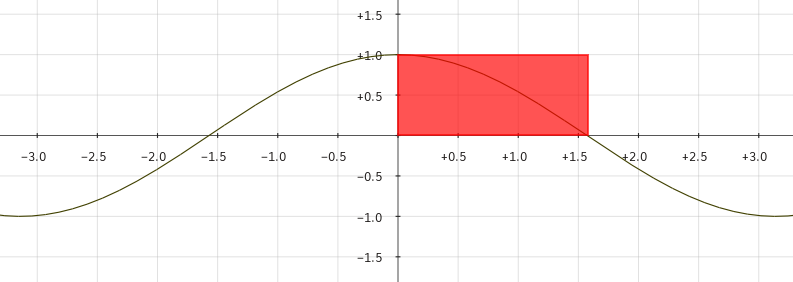
\includegraphics[width=0.8\textwidth]{img/coseno.png}
  \caption{Comportamiento de la función $\cos$. En rojo la región que involucra nustros resutlados}
  \label{bus:img-coseno}
\end{figure}
Si bien la función es circular, en nuestro problema particular solo nos centramos en un área de ella, ya que nuestros vectores solo pertenecen a un solo cuadrante del plano y además estan normalizados porque son porcentajes, con lo cuál sus componentes siempre serán positivas.\\
\begin{figure}[H]
  \centering
    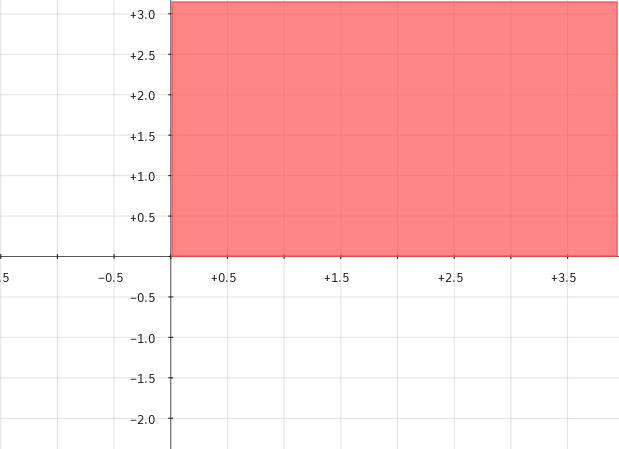
\includegraphics[width=0.4\textwidth]{img/planoCartesiano.png}
  \caption{Plano cartesiano. En rojo al cuadrante al que pertenecen nuestros vectores}
  \label{bus:img-planoCartesiano}
\end{figure}
De la anterior imágen podemos concluir que los ángulos que podemos obtener se encuentran limitados entre $0$\textdegree y $90$\textdegree, o lo que es lo mismo $0$ y $\frac{\pi}{2}$. De todo lo anterior obtenemos que:
$$0\leq \cos(\hat{\theta}) \leq 1$$
Como en la región que nos interesa la función $\cos$ es decreciente y su inversa $\arccos$ también lo es en el intervalo deseado $[0, 1]$. Entonces buscar el menor ángluo $\theta$ o su $\cos$ nos resulta igual.\\
Lo que nos llevó a definir que la similitud de dos vectores estará dada por el $\cos$ del ángulo que forman éstos y de esta manera introducimos menos errores de redondeo al no calcular la función.\\
Siempre que dos vectores tengan un ángulo cercano a $0$\textdegree más similares van a ser los papers. Eso lo podemos ver geometricamente porque vectores de este estilo son paralelos o sus pendientes son muy cercanas, haciendo que en muchos puntos la distancia entre ellos sea muy pequeña.  En nuestro problema particular, esto implicaría que en muchas de sus coordenas o temas a los que pertenece sus porcentajes son parecidos.\\
Ángulos cercanos a $90$\textdegree son ortogonales o muy diferentes ya que no tienen ningún atributo en común por lo que comparten temáticas entre ellos.
\section{Papers similares, diferentes conferencias}\label{bus:papSimDisLug}
El objetivo de esta búsqueda es generar una solución de bundles, en el que cada elemento contenga 
papers de tópicos similares pero que se hayan presentado en distintas conferencias.\\
Para realizar esta búsqueda se debe definir que se entiende por papers de tópicos similares y cual 
es la presentación de la conferencia. Para ello en la base de datos \cite{dataDrive} cuenta 
con la información de la presentación del paper, \texttt{venue} de ahora en adelante, y los 
perfiles de cada paper, \texttt{topicProfile} a partir de ahora.\\
La primer característica se utilizó para la complementariedad de dos papers, por lo que en cada 
bundle no habrá dos papes de un mismo \texttt{venue}. Cada paper se representó
con un vector de dimensión $N$ en el que el valor de cada elemento es el porcentaje del \texttt{topicProfile}.\\ 
La función de similitud se define como la distancia angular entre los vectores.
\section{Autores similares, distintas universidades}
Esta búsqueda consiste en encontrar una solución de bundles en el que cada bundle contiene autores 
similares pero de distinta universidad de afiliación.\\
Para determinar la similitud entre los autores se creó un perfil de cada uno. Para lograrlo lo 
primero que se hizo fue tener en cuenta todos los perfiles de papers en los que participaron cada 
uno de ellos. Al igual que con los papers, el perfil de los autores se representó con un vector. 
Este vector se cálculo sumarizando los vectores de cada uno de los papers en el que participó.\\
Para la función de similitud se utilizaron dos definiciones. La primera, al igual que con los papers,
consiste en la distancia angular. La otra definición es calcular la norma del vector resultante de la resta
vectorial entre los vectores de cada autor.\\
La complementariedad de dos papers se definió al lugar de pertenencia del autor en cuestión.
\section{Papers similares, con un perfil específico}
A la búsqueda de ``papers similares de diferente conferencia'' se le agregó una variante para ponderar
soluciones que contengan \texttt{topicProfile} específicos.
Para ello se agregó un parámetro que con el porcentaje de cada \texttt{topicProfile} para la ponderación.
Encontrar una solución de bundles de manera similar a ~\ref{bus:papSimDisLug} teniendo en cuenta que cada 
bundle además de compartir sus similitudes, también deben guardar relación con los tópicos 
específicos.\\
\section{Instituciones similares, diferentes regiones}
En este caso, la búsqueda es para instituciones similares de diferentes regiones. Al igual que con las 
búsquedas de autores, el perfil de cada institución se determino a partir del \texttt{topicProfile} de los papers
de estas. La complementariedad por la el atributo de la región de la institución. 
Luego el procedimiento para buscar soluciones, fue idéntico al utilizado para el de los autores.